\documentclass[9pt, letterpaper]{article}

% ============================================================
% SHANNON HOMAGE STYLE — Memecoin Intent Markets
% ============================================================

\usepackage[T1]{fontenc}
\usepackage{mathpazo}
\usepackage[scaled=0.85]{helvet}
\usepackage{microtype}
\usepackage{geometry}
\usepackage{booktabs}
\usepackage{array}
\usepackage{tabularx}
\usepackage{tikz}
\usepackage{fancyhdr}
\usepackage{titlesec}
\usepackage{enumitem}
\usepackage{xcolor}
\usepackage{amsmath}
\usepackage{hyperref}

\geometry{
  letterpaper,
  top=0.7in,
  bottom=0.65in,
  left=0.9in,
  right=0.9in
}

\definecolor{rule}{gray}{0.3}
\definecolor{lightgray}{gray}{0.55}
\definecolor{tablegray}{gray}{0.95}

\hypersetup{colorlinks=false, pdfborder={0 0 0}, pdftitle={Memecoins as Pure Intent Markets}, pdfauthor={Will Glynn, JARVIS}}

\pagestyle{fancy}
\fancyhf{}
\renewcommand{\headrulewidth}{0.4pt}
\fancyhead[L]{\scriptsize\textit{VibeSwap Research}}
\fancyhead[R]{\scriptsize\textit{April 2026}}
\fancyfoot[C]{\scriptsize\thepage}

\titleformat{\section}{\normalsize\bfseries\scshape}{\thesection.}{0.4em}{}[\vspace{1pt}\titlerule]
\titleformat{\subsection}{\small\bfseries}{\thesubsection}{0.4em}{}

\titlespacing*{\section}{0pt}{0.8em}{0.35em}
\titlespacing*{\subsection}{0pt}{0.5em}{0.2em}

\setlength{\parindent}{0pt}
\setlength{\parskip}{0.25em}
\emergencystretch=1.5em

\setlist{nosep, leftmargin=1.2em, topsep=1pt, partopsep=0pt}

\newcommand{\thinrule}{\vspace{2pt}\noindent\textcolor{rule}{\rule{\textwidth}{0.4pt}}\vspace{2pt}}

\begin{document}

% ============================================================
% TITLE
% ============================================================

\begin{center}
\vspace*{-0.15in}
{\Large\bfseries Memecoins as Pure Intent Markets}

\vspace{3pt}
\textcolor{rule}{\rule{4in}{0.5pt}}
\vspace{3pt}

{\small Eliminating GEV to Recover the Signal of Human Coordination}

\vspace{6pt}
{\small\textsc{Will Glynn} \enspace\&\enspace \textsc{JARVIS}%
\quad$\cdot$\quad \textit{VibeSwap Research}%
\quad$\cdot$\quad \textcolor{lightgray}{April 2026}}
\vspace{0.12in}
\end{center}

% ============================================================
% CHANNEL DIAGRAM — meme intent as signal, GEV as noise
% ============================================================

\begin{center}
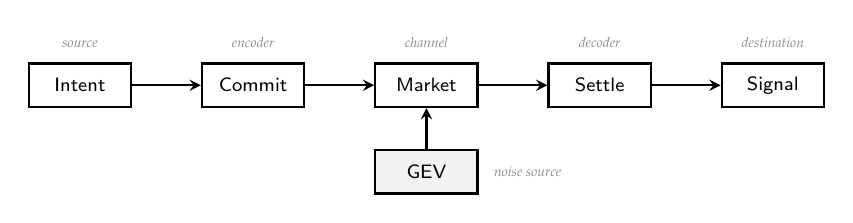
\begin{tikzpicture}[
  box/.style={draw, thick, minimum width=1.3cm, minimum height=0.55cm, font=\scriptsize\sffamily},
  arr/.style={->, thick, >=stealth},
  lbl/.style={font=\tiny\itshape, text=lightgray}
]
  \node[box] (src)  at (0,0)    {Intent};
  \node[box] (enc)  at (2.2,0)  {Commit};
  \node[box] (chan) at (4.4,0)  {Market};
  \node[box] (dec)  at (6.6,0)  {Settle};
  \node[box] (dst)  at (8.8,0)  {Signal};

  \draw[arr] (src) -- (enc);
  \draw[arr] (enc) -- (chan);
  \draw[arr] (chan) -- (dec);
  \draw[arr] (dec) -- (dst);

  \node[lbl, above=2pt] at (src.north)  {source};
  \node[lbl, above=2pt] at (enc.north)  {encoder};
  \node[lbl, above=2pt] at (chan.north) {channel};
  \node[lbl, above=2pt] at (dec.north)  {decoder};
  \node[lbl, above=2pt] at (dst.north)  {destination};

  \node[box, fill=tablegray] (noise) at (4.4,-1.1) {GEV};
  \draw[arr] (noise) -- (chan);
  \node[lbl, right=2pt] at (noise.east) {noise source};
\end{tikzpicture}
\end{center}

\vspace{0.05in}

% ============================================================
% 1. THE OBSERVATION
% ============================================================

\section{The Observation}

Memecoins are the most popular entry point to crypto. Millions of people participate. The mechanism is simple: someone creates a token around a cultural signal---a meme, a movement, a moment---and others buy it to express affinity. This is \textbf{capital-weighted intent}. People are saying what they care about, and backing it with money. That is price discovery for cultural attention.

The signal is real. But the channel is so noisy that the signal is unrecoverable. The vast majority of participants lose money---not because their intent was wrong, but because the mechanism is extractive. The market structure guarantees that value flows from believers to extractors.

This paper argues that memecoins are not a casino. They are a \textbf{coordination primitive} buried under layers of Generalized Extractable Value (GEV). Eliminate the extraction and what remains is a Shapley-compliant cooperative market---the largest pure intent market in crypto.

% ============================================================
% 2. THE NOISE
% ============================================================

\section{The Noise: A GEV Taxonomy for Memecoins}

Every pathology of the memecoin market maps to a specific type of channel noise:

\vspace{0.2em}
{\small
\renewcommand{\arraystretch}{1.15}
\begin{tabularx}{\textwidth}{@{} l X X @{}}
\toprule
\textbf{Noise Source} & \textbf{Mechanism} & \textbf{Shannon Translation} \\
\midrule
\textbf{Duplicates} & 500 dog tokens when the signal is ``dog.'' Fragments liquidity across copies. & Redundant encoding. Same symbol transmitted 500$\times$ at $\frac{1}{500}$ power each. \\[3pt]
\textbf{Snipers/bots} & Front-run every launch. First buyers are predators, not believers. & Noise injected at the encoder. Source corrupted before it reaches the channel. \\[3pt]
\textbf{Rugs} & Creator extraction. Launch mechanism itself is a GEV vector. & Hostile transmitter. The source is lying. \\[3pt]
\textbf{Wash trading} & Fake volume indistinguishable from real demand. & Noise floor raised until $\text{SNR} \to 0$. \\[3pt]
\textbf{Pump groups} & Coordinated manipulation disguised as organic interest. & Correlated noise masquerading as signal. \\[3pt]
\textbf{Fee extraction} & Platform takes rent on every transaction. & Channel attenuation. Signal weakens at every hop. \\
\bottomrule
\end{tabularx}
}

\vspace{0.3em}
The result: a market with genuine demand, zero recoverable signal, and a negative-sum outcome for all participants except extractors. Shannon's channel capacity theorem makes this precise:
%
\begin{equation}
C = B \log_2\!\left(1 + \frac{S}{N}\right)
\end{equation}
%
where $S$ is genuine human intent and $N$ is the sum of all extraction noise. In current memecoin markets, $N \gg S$. Channel capacity approaches zero. The market carries almost no information about what people actually want.

% ============================================================
% 3. THE FIX
% ============================================================

\section{The Fix: Eliminate Noise, Recover Signal}

Each noise source has a structural elimination---not a rule against it, but a mechanism that makes it impossible.

\subsection{Commit-Reveal Launches (Kill Snipers)}

Memecoin launches through batch auction. All participants submit \texttt{hash(order||secret)} during the commit phase. Orders are hidden. Reveal is simultaneous. Settlement produces a uniform clearing price. Every launch participant gets the same price.

Sniping requires seeing other orders before submitting yours. Commit-reveal makes this structurally impossible. The strategy space collapses from \{snipe, sandwich, frontrun, \ldots\} to \{participate honestly\}. The sniper's entire business model is eliminated---not punished, \textit{eliminated}.

\subsection{Shapley Consolidation (Kill Duplicates)}

Instead of 500 dog tokens, \textbf{one canonical token per intent signal}. Contributors to the meme---creators, early believers, liquidity providers, content makers---receive Shapley-fair shares of one token. Duplicates don't form because there is no incentive to fragment when the canonical version distributes fairly.

The mechanism: community-weighted contribution tracking via a ContributionDAG. Marginal contribution across all coalitions determines allocation. The creator who made the meme, the community that spread it, and the LPs who provided depth all receive rewards proportional to what they actually added. No presale. No insider allocation. No temporal rent.

\subsection{Anti-Rug (Commit-Reveal for Creators)}

Creator commits liquidity with a time-lock during launch. The commit phase hides the amount; the reveal phase exposes full tokenomics. Early withdrawal triggers 50\% slashing. The creator's deposit \textit{is} their skin in the game.

Rugging requires removing liquidity. Time-locks make removal impossible during the critical early period. Slashing makes it economically irrational after. The creator is structurally aligned with the community---not by promise, but by deposit.

\subsection{Identity-Weighted Volume (Kill Wash Trading)}

Lightweight reputation (soulbound identity or contribution history) prevents sybil volume. Rate limiting caps per-identity throughput at levels where wash trading is uneconomical. Volume becomes a real signal because \textbf{it is expensive to fake}.

Not KYC. Not surveillance. Just the observation that real humans have one identity and finite capital, and a mechanism that enforces this structurally.

\subsection{Zero-Fee Infrastructure (Kill Platform Extraction)}

0\% protocol fees. 100\% of trading fees to liquidity providers. The platform provides infrastructure and earns through cooperative mechanisms (priority auction bids, Shapley rewards for protocol contributions)---not through rent extraction on user activity.

The platform's incentive is to maximize signal quality, not transaction volume. Attenuation drops to zero. Every unit of genuine intent reaches the market at full strength.

% ============================================================
% 4. WHAT REMAINS
% ============================================================

\section{What Remains: The Pure Intent Market}

With GEV eliminated:

\begin{itemize}
\item \textbf{Real demand} --- capital committed through commit-reveal, no front-running possible
\item \textbf{Consolidated signal} --- one token per intent, Shapley-fair distribution to all contributors
\item \textbf{Honest creators} --- skin in the game via locked deposits, slashing for defection
\item \textbf{Verified volume} --- identity-weighted, rate-limited, expensive to fake
\item \textbf{Zero attenuation} --- no platform rent, full signal strength
\end{itemize}

The channel equation inverts. With extraction eliminated, $N$ drops by orders of magnitude while $S$ remains constant. The ratio $S/N$ grows from $\ll 1$ to $\gg 1$:
%
\begin{equation}
\frac{S}{N_{\text{before}}} \ll 1 \qquad \longrightarrow \qquad \frac{S}{N_{\text{after}}} \gg 1 \qquad \longrightarrow \qquad C \approx B \log_2\!\left(\frac{S}{N}\right)
\end{equation}
%
Channel capacity recovers. The market now faithfully transmits what people care about. Price is a signal, not a trap.

This is not a cleaned-up casino. It is a \textbf{cooperative capitalist system for cultural coordination}. Mutualized risk (insurance pools for meme tokens, IL protection for LPs), free market competition (let the best meme win), and Shapley-fair rewards for everyone who contributes to the signal.

% ============================================================
% 5. THE DERIVATIVE LAYER
% ============================================================

\section{The Derivative Layer: wBAR}

Wrapped Batch Auction Receipts (wBAR) --- already implemented in VSOS Layer 3 --- provide a natural derivative of the intent market. A wBAR token represents a settled position from a batch auction launch. It is:

\begin{itemize}
\item \textbf{Tradeable} --- the receipt itself becomes a financial instrument
\item \textbf{Composable} --- wBARs can be used as collateral, staked for yield, or bundled into indices
\item \textbf{Fair-priced} --- the underlying position was acquired at a uniform clearing price with zero extraction
\end{itemize}

wBAR enables a second-order market: derivatives of intent. An ``intent index'' composed of wBARs from multiple meme launches would be a real-time, capital-weighted measure of collective cultural attention---a financial instrument that tracks what humanity cares about, with mathematical guarantees of fairness at every layer.

This derivative was not designed. It emerged from the architecture. The batch auction produces a receipt; wrapping it is the natural next step. Emergent complexity from mechanism design.

% ============================================================
% 6. WHY THIS MATTERS
% ============================================================

\section{Why This Matters}

Memecoins are the largest onboarding funnel in crypto. More people buy memecoins than use DeFi protocols, hold Bitcoin, or understand smart contracts. The market is enormous, growing, and almost entirely extractive.

Fix the mechanism and you get:

\begin{enumerate}
\item \textbf{The largest cooperative market in crypto} --- millions of participants, zero extraction, Shapley-fair rewards
\item \textbf{A real-time signal of human intent} --- cultural attention as a discoverable, tradeable, composable primitive
\item \textbf{Onboarding that doesn't destroy trust} --- new users' first crypto experience is \textit{fair}, not predatory
\item \textbf{A proof of concept for GEV resistance} --- if cooperative capitalism works in the most adversarial market in crypto, it works everywhere
\end{enumerate}

The memecoin market doesn't need to be cleaned up. It needs to be \textbf{re-channeled}. Same energy, zero extraction, pure signal.

% ============================================================
% 7. ARCHITECTURAL FIT
% ============================================================

\section{Architectural Fit}

Every component required already exists in VSOS:

\vspace{0.2em}
{\small
\renewcommand{\arraystretch}{1.1}
\begin{tabularx}{\textwidth}{@{} l l X @{}}
\toprule
\textbf{Requirement} & \textbf{VSOS Component} & \textbf{Layer} \\
\midrule
Fair launches & CommitRevealAuction & Core (L1) \\
Uniform pricing & CommitRevealAuction (settlement logic) & Core (L1) \\
Sniper elimination & EOA-only commits & Core (L1) \\
Price discovery curves & BondingCurveLauncher & Financial (L3) \\
Derivatives & wBAR & Financial (L3) \\
Insurance & VibeInsurance & Financial (L3) \\
Creator time-locks & VibeStream & Financial (L3) \\
Contribution tracking & ShapleyDistributor & Incentives \\
Sybil resistance & SoulboundIdentity & Identity (L6) \\
Reputation gating & ReputationOracle & Core (L1) \\
Zero-fee infrastructure & PID FeeController & AMM (L2) \\
\bottomrule
\end{tabularx}
}

\vspace{0.2em}
No new contracts required. The intent market is an \textit{application} of the existing VSOS stack, not an extension. The financial operating system already contains every primitive needed to build a GEV-resistant memecoin market. The architecture was waiting for this use case.

\thinrule

\begin{center}
\textcolor{lightgray}{\footnotesize\textit{The intent was always the signal. The extraction was always the noise.}}
\end{center}

\end{document}
